\section{Audio}
\label{sec:audio}
The audio system is is responsible for playing sfx and music.
\begin{itemize}
    \item Sfx work in a 'fire and forget' way: a single function call to the AudioSource is required to start playing the sound, and it never needs to be stopped or cleaned up in any way. The engine stops playing the sfx when it is finished \footnote{Unless specified that the sound should loop}.
    \item Music can be played, stopped and adjusted while it is playing, however, just like sfc, music does not need to be manually stopped.
\end{itemize}

\subsection{Audio library}
As discussed in the research, it is best to use an audio library (rather than manually doing system calls)
, and there are many audio libraries to choose from. By trying out various audio libraries, it was concluded that
SDL Mixer is the best library to use for this engine. While it is not as extensive as other libraries,
it has the features to meet the engine requirements, and its ease of use makes it a sensible choice.

\subsection{Class diagram}
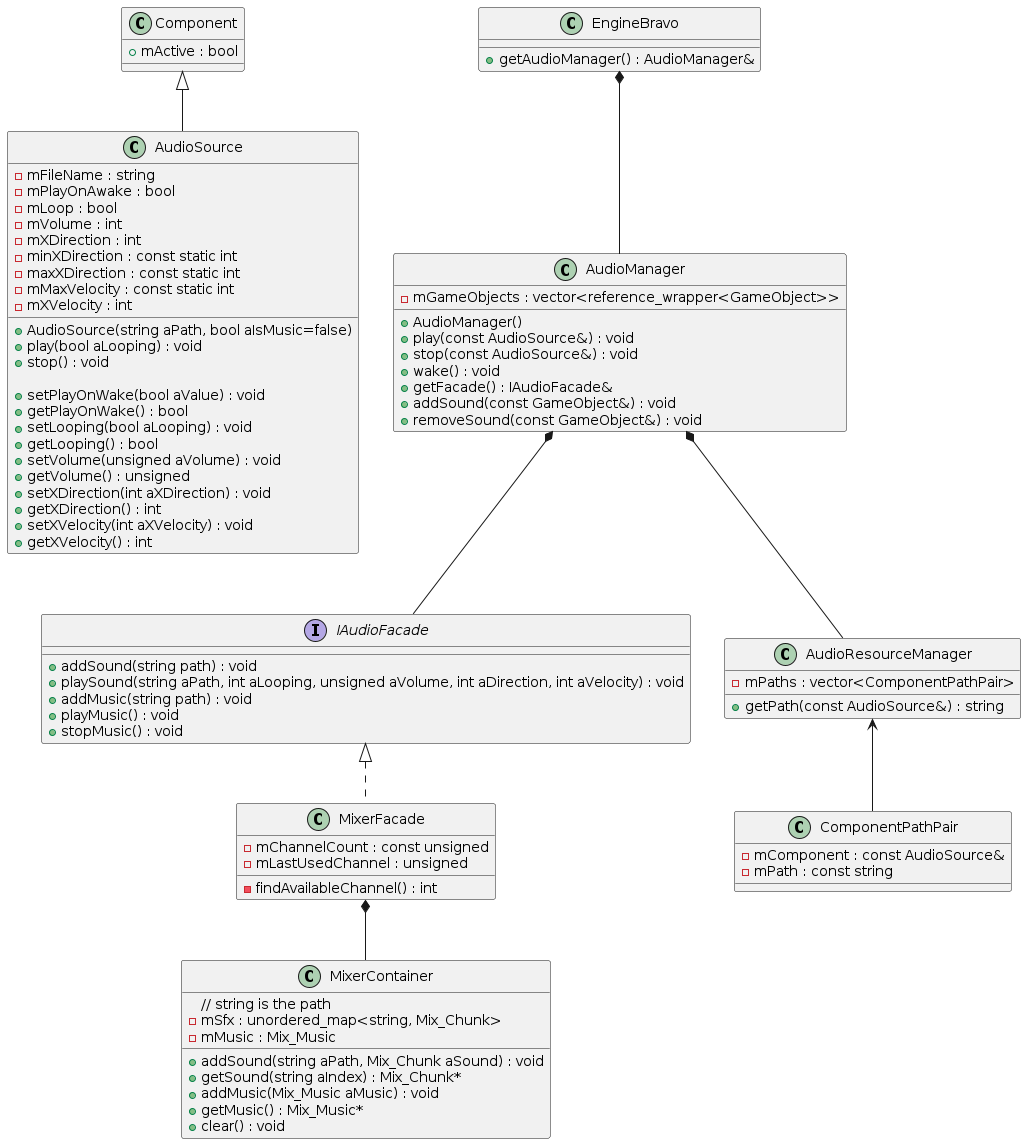
\includegraphics[width=\textwidth]{audioClassDiagram.png}
In the following subsections, the classes in this diagram are further detailed.

\subsubsection{IAudioFacade}
A facade interface to make the coupling between the AudioManager and the used audio library less tight.

\subsubsection{MixerFacade}
The implementation of the audio facade interface for SDL mixer.
Because channel \footnote{what is called a channel in SDL mixer is more commonly known as a track.} management is done
manually in SDL mixer, the mChannelCount and mLastUsedChannel variables are used to determine the next available channel for playing sfx.

\subsubsection{MixerContainer}
The mixer container holds all the
SDL mixer sound files.
The string in the mSfx map is the path to the file, because that can be considered as a sort of unique id for the sound file.